% TU Delft Beamer template
% Author: Maarten Abbink
% Delft University of Technology
% March 2014
% Version 2.0
% Based on original version 1.0 of Carl Schneider
\documentclass{beamer}
\usepackage[dutch]{babel}
\usepackage{calc}
\usepackage[absolute,overlay]{textpos}
\usepackage{amsmath}
\usepackage{amsthm}

\mode<presentation>{\usetheme{tud}}

\title[NedTrain Planner]{NedTrain Planner}
%\subtitle
\institute[TU Delft]{Technische Universiteit Delft}
\author{Chris Bakker, Anton Bouter, Martijn den Hoedt}
\date{2 juli 2014}

\theoremstyle{definition}
\newtheorem{definitie}{Definitie}[section]

% Insert frame before each subsection (requires 2 latex runs)
\AtBeginSubsection[] {
	\begin{frame}<beamer>\frametitle{\titleSubsec}
		\tableofcontents[currentsection,currentsubsection]  % Generation of the Table of Contents
	\end{frame}
}
% Define the title of each inserted pre-subsection frame
\newcommand*\titleSubsec{Next Subsection}
% Define the title of the "Table of Contents" frame
\newcommand*\titleTOC{Outline}

% define a symbol which can be removed if you don't need it
\newcommand{\field}[1]{\mathbb{#1}}
\newcommand{\Zset}{\field{Z}}

\begin{document}

{
% remove the next line if you don't want a background image
\usebackgroundtemplate{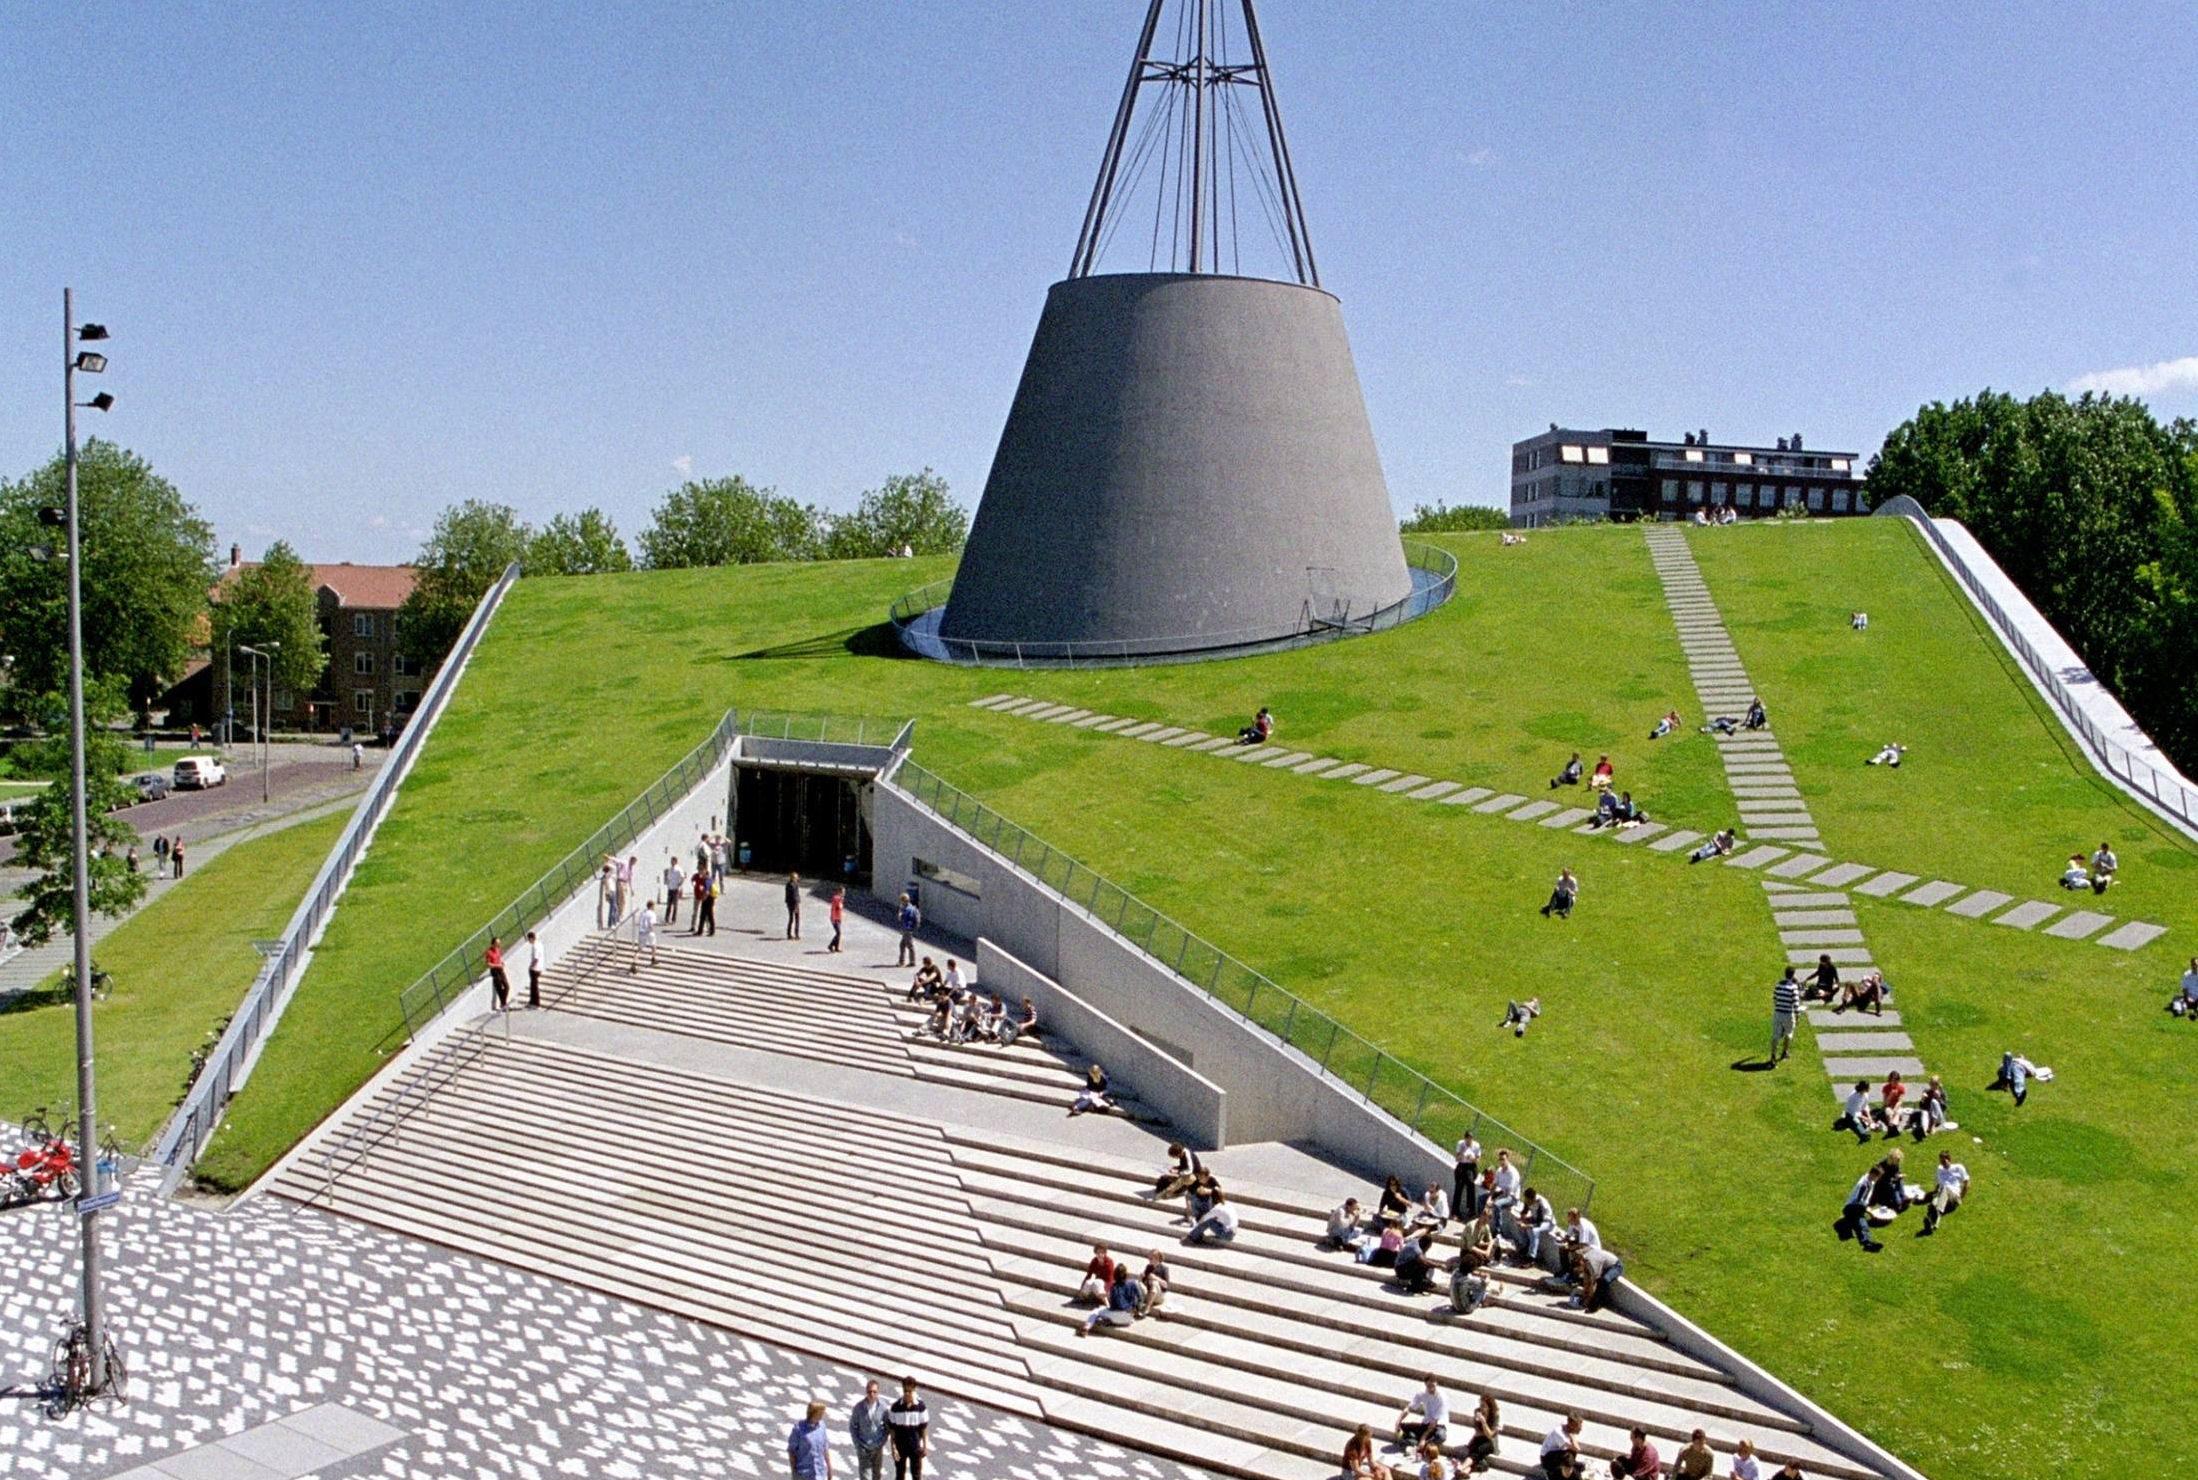
\includegraphics[width=\paperwidth,height=\paperheight]{images/background-titlepage.jpg}}%
\setbeamertemplate{footline}{\usebeamertemplate*{minimal footline}}
\frame{\titlepage}
}

\begin{frame}\frametitle{Opdrachtgevers}
\begin{columns}[T] % align columns
    \begin{column}{.55\textwidth}
        \begin{itemize}
            \item NedTrain 
            \begin{itemize}
                \item Nederlandse Spoorwegen
                \item $250$ treinen op $30$ locaties
                \item $3500$ werknemers
                \item ir. Bob Huisman
            \end{itemize}
        \end{itemize}
        \vspace{1.8cm}
        \begin{itemize}
            \item TU Delft
            \begin{itemize}
                \item Algoritmiek groep
                \item prof. dr. Cees Witteveen
            \end{itemize}  
        \end{itemize}
    \end{column}%
    \begin{column}{.45\textwidth}
        
\includegraphics[width=4.5cm]{images/logo-nedtrain.jpg}
        \vspace{1cm}
        
\includegraphics[width=5cm]{images/tudelft_logo.pdf}
    \end{column}%
\end{columns}
\end{frame}


\begin{frame}\frametitle{Linear Programming}
    \begin{definitie}
        \begin{align}
            \text{max:}& \quad \sum_{t \in T} (t^+ - t^-) & \nonumber \\
            % constraint 1
            \only<1>{\phantom{\text{met voorwaarden:}} & \phantom{\quad t^- \leq t^+} & \phantom{\forall t \in T} \nonumber \\}
            \only<2->{\text{met voorwaarden:} & \quad t^- \leq t^+ & \forall t \in T \nonumber \\} 
            % contraint 2
            \only<-2>{& \phantom{\quad a^+ - b^- \leq -d_a} & \phantom{\forall (a \prec b) \in C} \nonumber}
            \only<3-8>{& \phantom{\quad a^+ - b^- \leq -d_a} & \forall (a \prec b) \in C \nonumber}
            \only<9->{& \quad a^+ + d_a \leq b^- & \forall (a \prec b) \in C \nonumber}
        \end{align}
    \end{definitie}

    \begin{itemize}
        \item \only<4->{$a \prec b$} \only<8->{$\quad \Rightarrow \quad a^+ + d_a \leq b^-$}
        \item<10-> COIN-OR Linear Programming Solver (CLP)
    \end{itemize}

    \begin{tikzpicture}
        \draw[very thick, visible on=<4->] (-0.4mm, 2.5mm) -- (100mm, 2.5mm);
        \draw[very thick, visible on=<4->] (-0.4mm, 0mm) -- (-0.4mm, 5mm);
        \draw[very thick, visible on=<4->] (100mm, 0mm) -- (100mm, 5mm);

        \filldraw[very thick, draw=darkgreen,fill=lightgreen, visible on=<4-5>] (0mm,0mm) rectangle (40mm,5mm) node[pos=.5] {$a$};
        \filldraw[very thick, draw=darkgreen,fill=lightgreen, visible on=<6->] (10mm,0mm) rectangle (50mm,5mm) node[pos=.5] {$a$};
        \filldraw[very thick, draw=darkyellow,fill=lightyellow, visible on=<4->] (50.4mm,0mm) rectangle (70mm,5mm) node[pos=.5] {$b$};

        \draw [decorate, decoration={brace,amplitude=10pt}, visible on=<5>]
        (0mm,6mm) -- (40mm,6mm) node [black,midway, yshift=6mm] 
        {\footnotesize $d_a$};
\draw [decorate, decoration={brace,amplitude=10pt}, visible on=<6->]
        (10mm,6mm) -- (50mm,6mm) node [black,midway, yshift=6mm] 
        {\footnotesize $d_a$};

        \node[visible on=<5->] at (0mm, -2mm) {$a^-$};
        \node[visible on=<7->] at (10mm, -2mm) {$a^+$};
        \node[visible on=<5->] at (50mm, -2mm) {$b^-$};
    \end{tikzpicture}
\end{frame}

\begin{frame}\frametitle{Demo}
    \huge{\hfill Tijd voor een demo! \hfill}
\end{frame}


\end{document}
